Vestibulum et arcu ex. Duis imperdiet placerat suscipit. Nulla scelerisque, tortor a fringilla iaculis, tellus lacus sagittis ex, non molestie purus ex in dolor. Nulla purus metus, varius in ante in, rutrum vulputate sem. Curabitur eget suscipit tellus. Nulla ut feugiat nisl. Integer velit est, porttitor eget metus eu, mollis sagittis augue. Fusce ac purus luctus, faucibus tellus eget, elementum orci. Phasellus non feugiat elit, sed aliquet nibh. Sed vehicula sit amet leo id faucibus. Ut iaculis orci quis dapibus viverra. Donec maximus blandit ante. Nullam vehicula felis a ante suscipit, a finibus purus facilisis. Nullam interdum urna ipsum.

\section{Sistema MIMO}
Nulla condimentum euismod purus. Sed justo purus, mollis vel erat at, eleifend vehicula ligula. Aenean finibus eleifend eros, ac placerat justo porta eu. Nunc mattis eu metus sed ornare. Suspendisse orci tortor, porta maximus efficitur vitae, pretium at turpis. Aliquam gravida faucibus aliquam. Mauris porta mi eget odio pretium congue. Class aptent taciti sociosqu ad litora torquent per conubia nostra, per inceptos himenaeos.
\\
\\
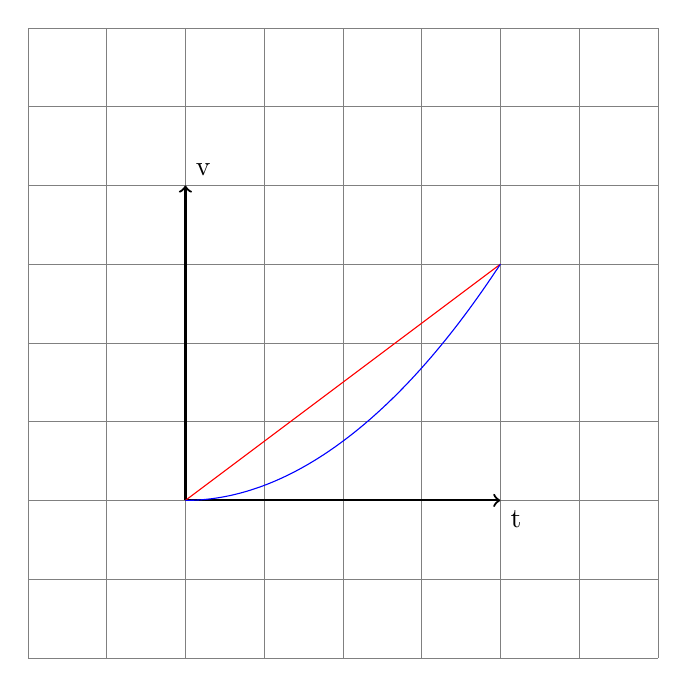
\begin{tikzpicture}

    \draw [step=1cm, gray, very thin] (-2,-2) grid (6,6);
    \draw[thick, ->] (0,0) -- (4,0)
    node[anchor=north west] {t};
    \draw[thick, ->] (0,0) -- (0,4)
    node[anchor=south west] {v};
    
    \draw[red] (0,0) -- (4,3);
    \draw[blue] (0,0) parabola (4,3);

\end{tikzpicture}
\\
\\
Nulla condimentum euismod purus. Sed justo purus, mollis vel erat at, eleifend vehicula ligula. Aenean finibus eleifend eros, ac placerat justo porta eu. Nunc mattis eu metus sed ornare. Suspendisse orci tortor, porta maximus efficitur vitae, pretium at turpis. Aliquam gravida faucibus aliquam. Mauris porta mi eget odio pretium congue. Class aptent taciti sociosqu ad litora torquent per conubia nostra, per inceptos himenaeos.
\\
\\
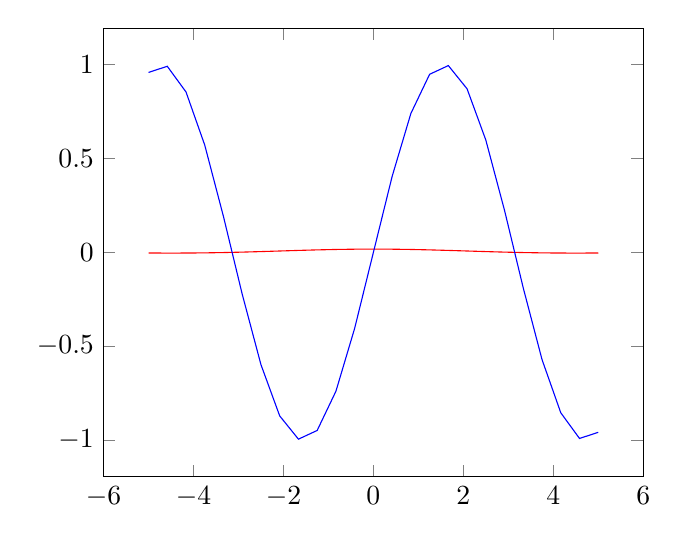
\begin{tikzpicture}
    \begin{axis}
        \addplot[color=red] {sin(deg(x))/deg(x)};
        \addplot[color=blue]{sin(deg(x))};
    \end{axis}
\end{tikzpicture}

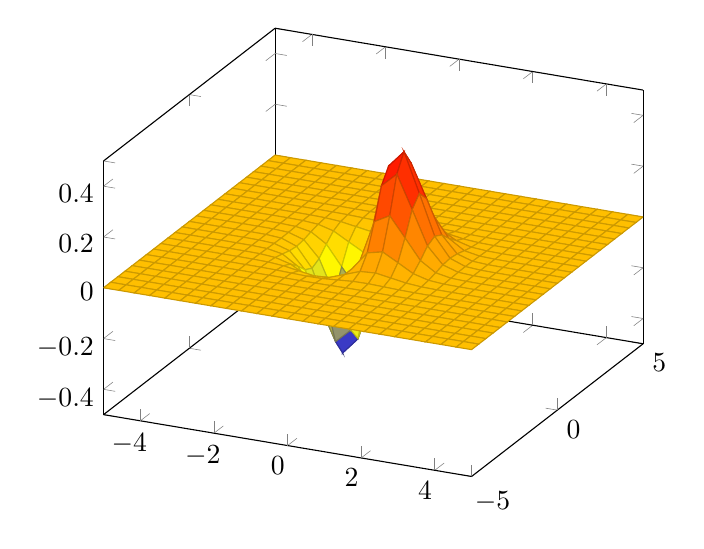
\begin{tikzpicture}
    \begin{axis}
        \addplot3[surf,]{exp(-x^2-y^2)*x};
    \end{axis}
\end{tikzpicture}
\\
\\
Nulla condimentum euismod purus. Sed justo purus, mollis vel erat at, eleifend vehicula ligula. Aenean finibus eleifend eros, ac placerat justo porta eu. Nunc mattis eu metus sed ornare. Suspendisse orci tortor, porta maximus efficitur vitae, pretium at turpis. Aliquam gravida faucibus aliquam. Mauris porta mi eget odio pretium congue. Class aptent taciti sociosqu ad litora torquent per conubia nostra, per inceptos himenaeos.
\\
\\
\begin{circuitikz}
\draw
(0,0) to[battery, V = $x \ V$] (0,4)
to[ammeter, i_=2$mA$](4,4)
to[C=3$F$] (4,0) -- (3.5, 0)
to[lamp, *-*] (0.5, 0) -- (0,0)
(0.5, 0) -- (0.5, -2)
to[voltmeter, l=3] (3.5, -2) -- (3.5, 0);
\end{circuitikz}